\section{Results}
\subsection{Relaxation time}
The variation of parameter $\tau$ in the spin-echo and 180°-90° sequence allowed us to measure the time evolution of the transverse, Fig. \ref{fig:GD500 T2 Sp} \& Fig. \ref{fig:GD600 T2 Sp}, and anti-parallel magnetization, Fig. \ref{fig:GD500 T1} \& Fig. \ref{fig:GD600 T1}. A second measurement for the transverse component using the Carr-Purcell sequence delivered Fig. \ref{fig:GD500 T2 CP} \& Fig. \ref{fig:GD600 T2 CP}. 

\begin{figure}[!htbp]
  \centering
  \begin{subfigure}[b]{0.45\textwidth}
    \centering
    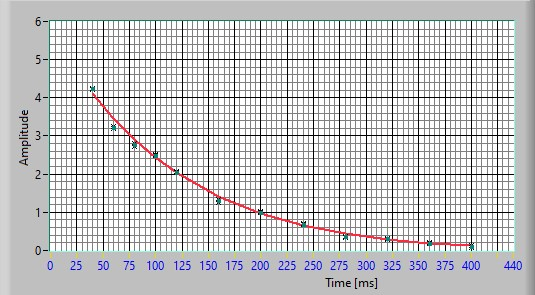
\includegraphics[width=\textwidth]{./Protocol images/GD500_T2_sp_fit (1).jpg}
    \caption{GD500}
    \label{fig:GD500 T2 Sp}
  \end{subfigure}
  \hfill
  \begin{subfigure}[b]{0.45\textwidth}
    \centering
    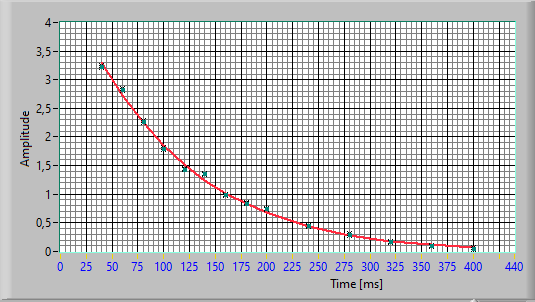
\includegraphics[width=\textwidth]{./Protocol images/GD60_Sp (1).png}
    \caption{GD600}
    \label{fig:GD600 T2 Sp}
  \end{subfigure}
  \caption{Decay curve of $M_\perp$ measured with spin-echo methode}
  \label{fig:subsidebyside}
\end{figure}

\begin{figure}[!htbp]
  \centering
  \begin{subfigure}[b]{0.45\textwidth}
    \centering
    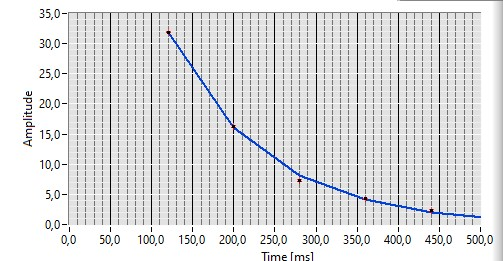
\includegraphics[width=\textwidth]{./Protocol images/GD500_T2_cp_fit.jpg}
    \caption{GD500}
    \label{fig:GD500 T2 CP}
  \end{subfigure}
  \hfill
  \begin{subfigure}[b]{0.45\textwidth}
    \centering
    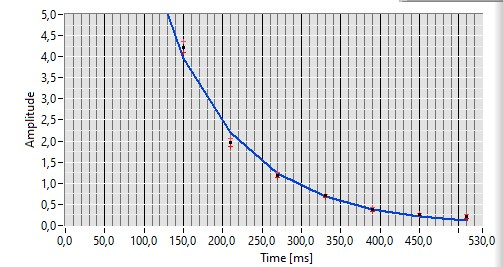
\includegraphics[width=\textwidth]{./Protocol images/GD600_CP_fit (1).jpg}
    \caption{GD600}
    \label{fig:GD600 T2 CP}
  \end{subfigure}
  \caption{Decay curve of $M_\perp$ measured with Carr-Purcell sequence}
  \label{fig:subsidebyside}
\end{figure}

\begin{figure}[!htbp]
  \centering
  \begin{subfigure}[b]{0.45\textwidth}
    \centering
    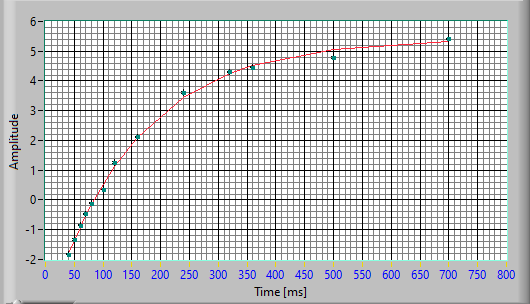
\includegraphics[width=\textwidth]{./Protocol images/GD500_T1 (1).png}
    \caption{GD500}
    \label{fig:GD500 T1}
  \end{subfigure}
  \hfill
  \begin{subfigure}[b]{0.45\textwidth}
    \centering
    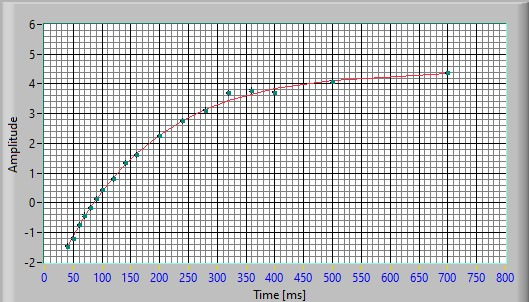
\includegraphics[width=\textwidth]{./Protocol images/GD600_T1 (1).jpg}
    \caption{GD600}
    \label{fig:GD600 T1}
  \end{subfigure}
  \caption{Decay curve of $M_\parallel$ measured with 180°-90° sequence}
  \label{fig:subsidebyside}
\end{figure}
A quick glance at the curves already tell  us that the time evolution of the components of the magnetization describe a decay curves, as we expected from the solutions of the bloch equations,  eq.\ref{eq: sol. bloch T1} \& eq. \ref{eq: sol. bloch T2}. By fitting these equation to our data we are able to find the characteristic relaxation times $T_1$ and $T_2$. See Tab. \ref{tab: relaxation times}.
\begin{table}[!htbp]
 \begin{center}
  \caption{Relaxation times for Gd500 and Gd600}
  \label{tab: relaxation times}
  \begin{tabular}{|c||c|c|c|c|}
	\hline
	\multirow{2}{*}{\textbf{Probe}} & \multicolumn{3}{c}{spin-spin $T_2$ [ms]} &\multirow{2}{*}{ spin-lattice $T_1$[ms]}\\
	& spin-echo & Carr-Purcell & deviation $\sigma$\\
	\hline
	\hline	
	Gd 500 & 110 $\pm$ 6 & 111,3 $\pm$ 1,5 & 0,5 & 159 $\pm$ 1,3 \\
	Gd 600 & 115,7 $\pm$ 1,2 & 116,9 $\pm$ 0,9 & 0,8 & 154,4 $\pm$ 1,2 \\
	\hline
  \end{tabular}
 \end{center}
\end{table}

The first observation we take from our results is that the spin-spin relaxation time of the probe with higher density, GD600, is larger than that of GD500, which contradicts our expectations. From our theory we know that $T_2$ is mainly determined by the interaction between the proton's spins. Hence the bigger the concentration, which translates to a larger amount of protons therefore of spins, the  more possibilities there exist for a proton to dissipate its excitation energy resulting in a smaller spin-spin relaxation time. 
%mention T1 measurements

From our experiment we can observe that the deviation between the results gained by the spin-echo and Carr-Purcell methods are not significant, however from our theory we know that this second method delivers more exact results. The Carr-Purcell sequence is also a faster measurement technique since it can be completely automatized, thus reducing the susceptibility to human errors. Lastly we also observe a higher precision from this second method, it delivers a smaller uncertainty in all measurements. This last point is better observed by the measurements of Gd500 where the uncertainty of the spin-echo method is almost 4 times bigger than the one delivered by the Carr-Purcell sequence. 
\subsection{Chemical shift}

\subsubsection{Imaging}
\paragraph{1 dimensional imaging}
\paragraph{Time evolution of system}
\paragraph{2 dimensional imaging}